\chapter{Simulações}   
\label{cap:III}
\section{Introdução}
 Definido o método dos elementos finitos com a formulação de Galerkin, temos diferentes meios para resolver o problema. Anteriormente resolvemos uma equação diferencial usando elementos finitos com \textbf{equações lineares}. Discretizando o espaço em elementos de tamanho \textbf{h} e utilizando as técnicas de derivação e integração numérica utilizando polinômios de grau \textbf{p}, podemos utilizar a combinação desses métodos nos fornece aproximações com erros menores, para diferentes métodos.
 
 Neste capítulo mostrarei resoluções de algumas equações diferenciais comparando os métodos \emph{h} e \emph{p}  e também aproximações por interpolações de funções utilizando pontos equidistantes e de Chebyshev. Todas as figuras e resoluções foram obtidas utilizando a linguagem de programação \emph{Julia}.

\section{Convergência do erro de interpolação utilizando o método espectral}
	Vamos agora ver a convergência do erro da aproximaçãode uma função de runge $\frac{1}{1+x^2},\ x\ \in [-5,5]$, para pontos \emph{equidistantes} e pontos igualmente espaçados, utilizando o polinômio de \textbf{Lagrange}.
	As aproximadas obtidas para raízes equidistantes e raízes de chebishev são mostradas na figura \ref{fig:interp}.	
\begin{figure}[!ht]
  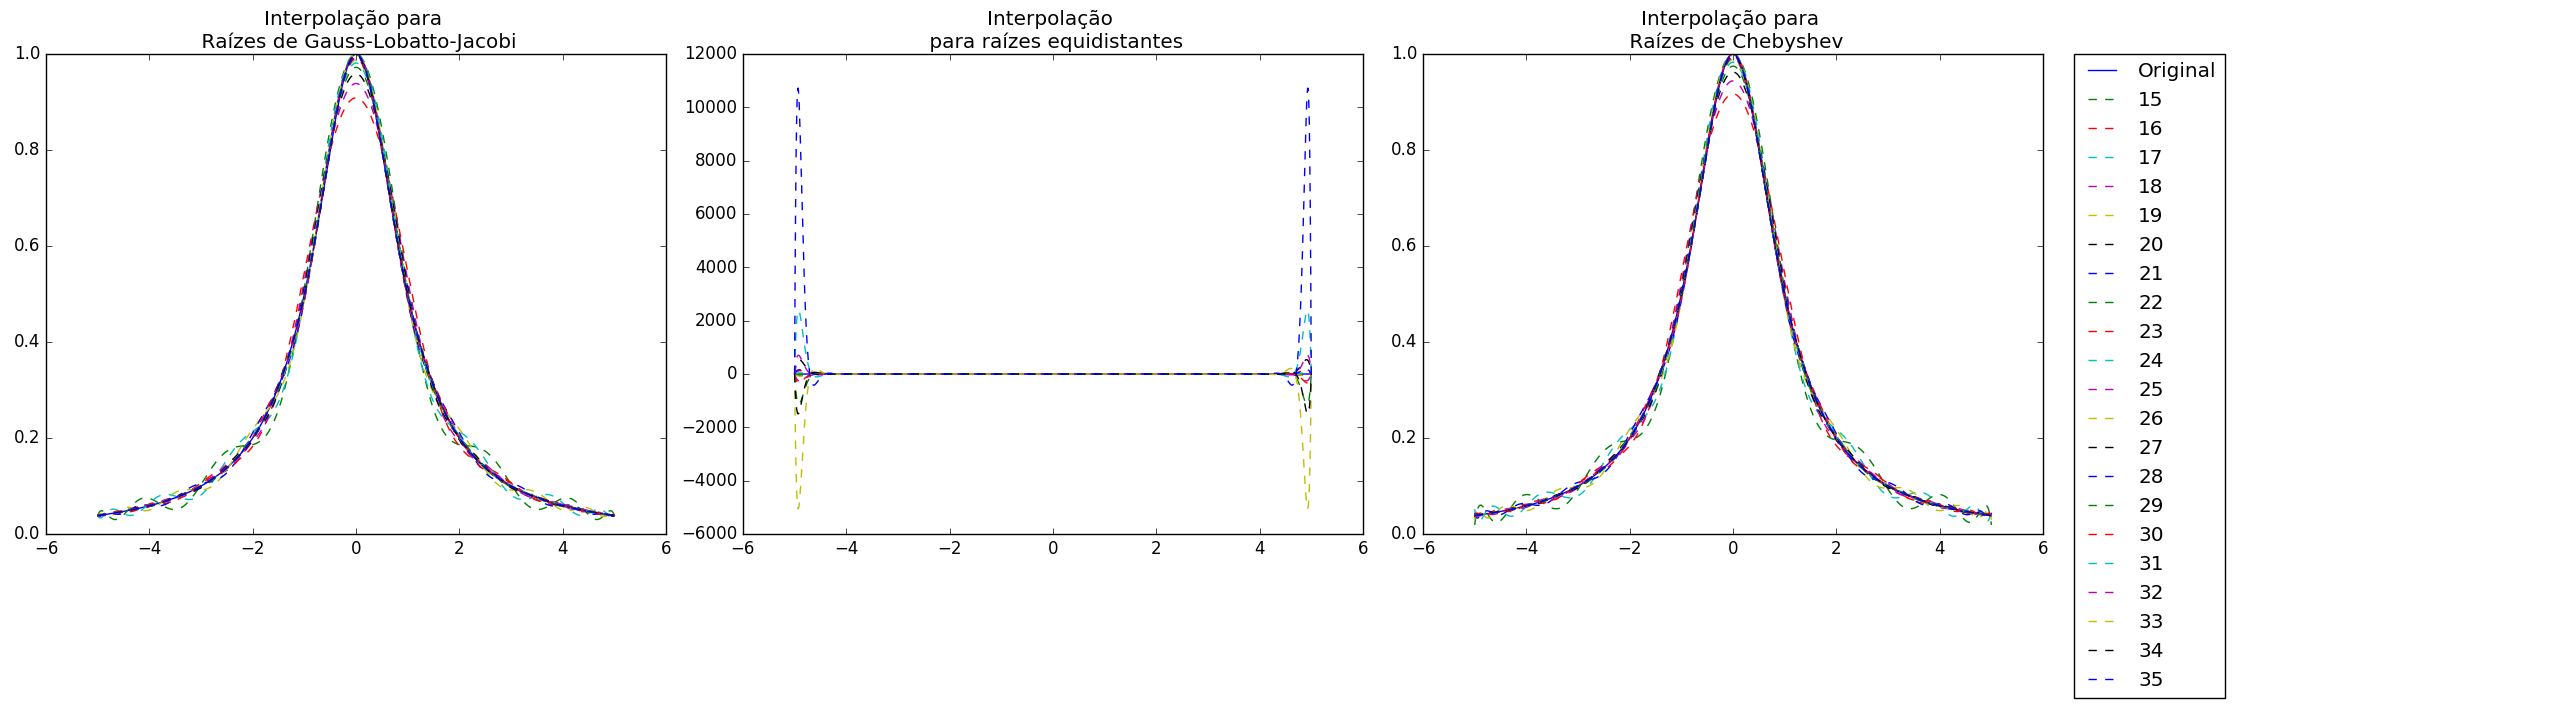
\includegraphics[width=1.25\textwidth,center]{figuras/interpolacao_todas.png}
  \caption{interpolação de polinômios de alta ordem com raízes de Gauss-Lobatto-Jacobi, igualmente espaçados, Chebyshev}
\label{fig:interp}
\end{figure}

Notamos novamente que para diferentes  polinômios de lagrange de alta ordem utilizando pontos igualmente espaçados, a aproximação nos pontos próximos das extremidades apresenta um erro  grande, enquanto que para pontos distribuídos usando as raízes de Chebyshev e de Gauss-Lobatto-Jacobi se comportam bem nessas regiões. Agora, iremos verificar a convergência desse erro, analizando o erro máximo para cada escolha de raízes.

Comparando as escolhas de raízes dos problemas conseguimos ver que a convergência do erro usando as raízes equidistantes aumenta conforme o grau do polinômio aumenta. Enquanto que para as raízes de Chebyshev e Gauss-Lobatto-Jacobi, os erros convergem algebricamente. 
\begin{figure}[!ht]
  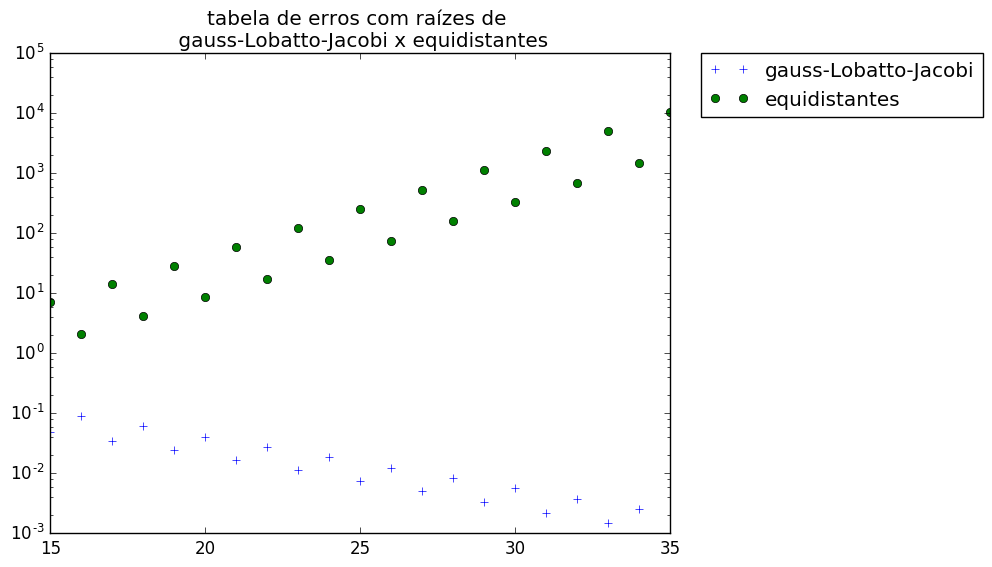
\includegraphics[width=0.8\textwidth,center]{figuras/glj_equi.png}
  \caption{comparação semilog  dos erros e graus de liberdade de raízes de glj versus equidistante }
\end{figure}
\begin{figure}[!hb]
  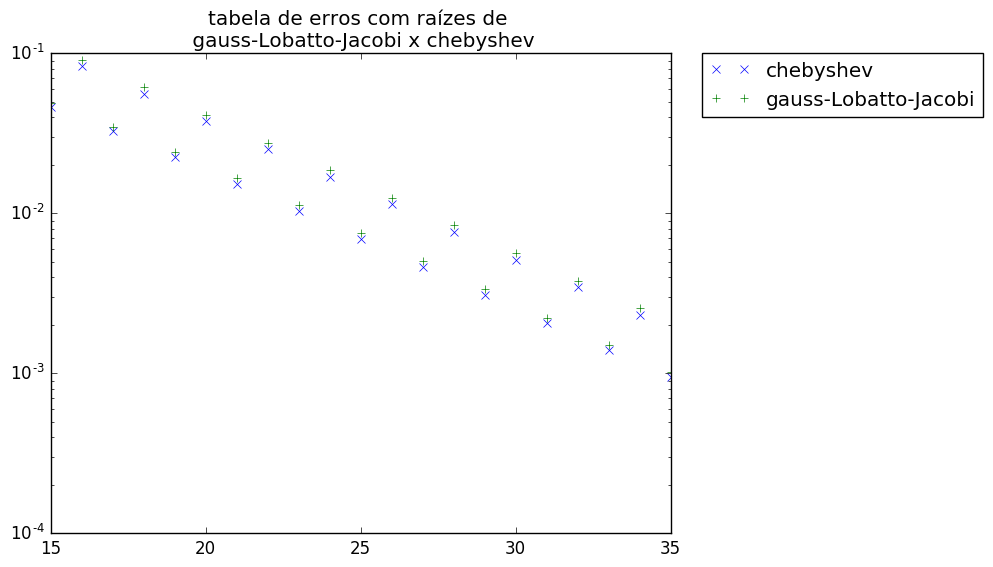
\includegraphics[width=0.8\textwidth,center]{figuras/glj_cheb.png}
  \caption{comparação semilog  dos erros e graus de liberdade de raízes de glj versus Chebyshev}
\end{figure}
\\
Notamos que embora a convergência, utilizando ambas as raízes dos polinômios, tenham o mesmo comportamento, podemos observar que como demonstrado  anteriormente a escolha do Polinômio de Chebyshev é o que melhor aproxima a função do fenômeno de Runge observando uma inclinação menor do erro.

\subsection{Convergência do erro de interpolação utilizando método H}
 Tendo aproximado a função de runge acima, utilizaremos um novo método chamado método H,método no qual subdividimos o problema em $n$ elementos de tamanho $H$. Iremos comparar o efeito desse método contra o método espectral anterior utilizando as mesmas raízes de aproximação, Gauss-Lobatto-Jacobi.

\begin{figure}[H]
\centering
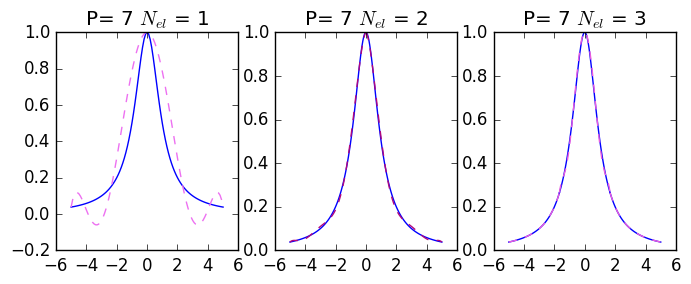
\includegraphics[width=0.7\textwidth,center]{figuras/interp_usando_FEM.png}
\caption{gráficos das aproximações fixado o grau do polinômio em 7 e subdividimos o domínio em $N_{el}$ elementos }
\end{figure}

\begin{figure}[H]
  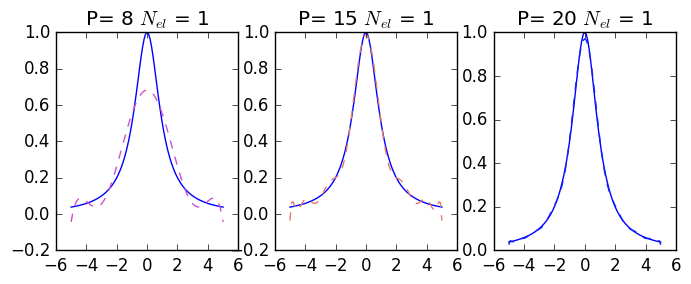
\includegraphics[width=0.8\textwidth,center]{figuras/interp_usando_FEMfixo.png}
  \caption{gráficos das aproximações fixado o número de elementos em 1 e utilizamos polinômios de grau elevado}
\end{figure}
 No gráfico de convergência do erro máximo, notamos que o decaimento para o método P é gemométrico enquanto para o método H é subgeométrico para o gráfico do tipo log-linear.
 \begin{figure}[H]
  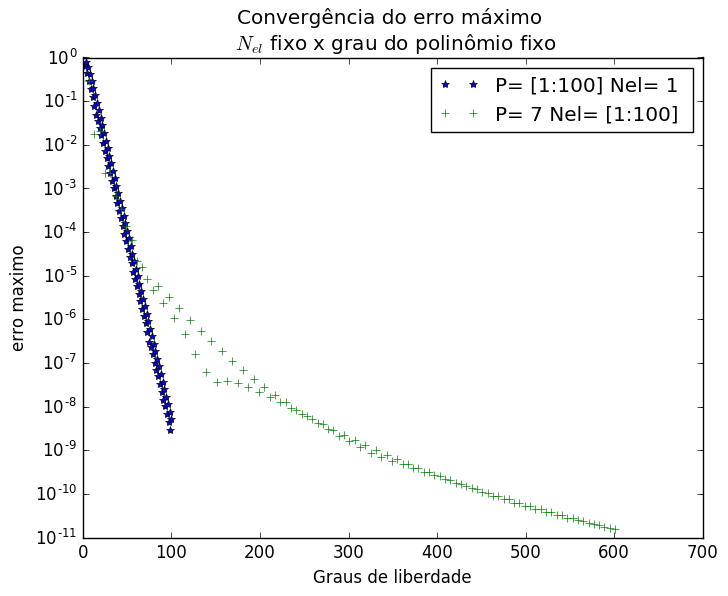
\includegraphics[width=0.7\textwidth,center]{figuras/convergencia_erro_FEM2.png}
  \caption{Convergência dos erros entre polinômios fixos e polinômios de grau elevado}
\end{figure}

\section{Método HP na resolução de equações diferenciais}

 Agora, resolveremos uma equação diferencial de segundo grau. Para tanto, irei apresentar uma equação com solução conhecida ($sin(2\ k \pi x)$). Nesse caso, definirei o problema com a condição de fronteira de \emph{Dirichlet}, definindo assim o valor nas extremidades do domínio. Abaixo, está um comparativo entre a solução exata e a solução aproximada do problema abaixo:
\begin{align}
y'' + y &= (1 + 4 (k \pi)^2)sin(2 k \pi x) \\
y(-1) &= sin(-2\ k \ \pi ) = 0 ,\ y(1) = sin(2\ k\ \pi) = 0 \ \ \forall k = 1,2,\dots \\
\end{align}	
\begin{figure}[H]
\centering
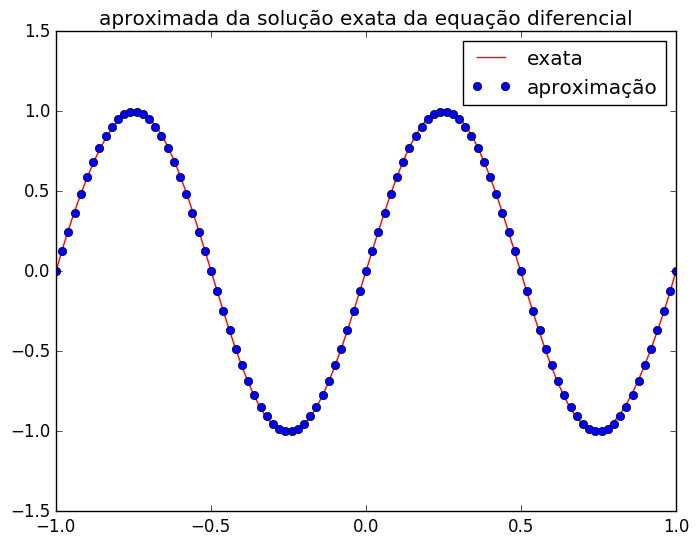
\includegraphics[width=0.5\textwidth,center]{figuras/solu_edo_simul.png}
\caption{comparação entre a solução exata e a aproximada usando P = 10 e $N_{el} = 10$ } 
\end{figure}
Na figura \ref{fig:convD} observamos  como o erro máximo varia para dois casos do Método \emph{HP}. No primeiro fixamos o grau P do polinômio interpolador e variamos o tamanho \emph{H} dos elementos, assim variando o número de elementos que discretizamos o problema. No segundo,  fixamos o número de elementos e variamos o grau do polinômio interpolador P.
\begin{figure}[H]
  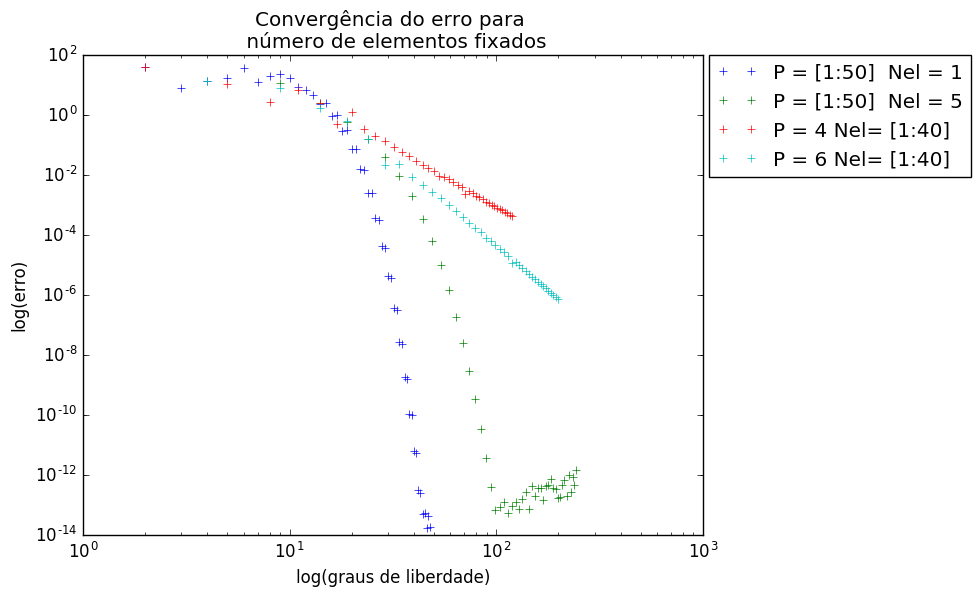
\includegraphics[width=.9 \textwidth,center]{figuras/convergencia_erro_HP.png}
  \caption{convergência do log(erro) em função dos log(graus de liberdade) comparando os métodos HP }
\label{fig:convD}
\end{figure}
 Novamente, notamos um decaimento maior quando fixamos o grau do polinômio e aumentamos o número de elementos do problema.
%\pagebreak
\subsection{Condição de Neumann}
 Agora utilizamos o método HP para um problema no qual temos em uma das extremidades uma condição de \emph{Neumann}. Nesse exemplo usarei como solução do problema $y(x) = \cos(10 x) \sin(25 x)$, onde $ x \in [-1,1]$ e a condição de Neuman está em $x=1$. Nesse caso temos que acrescentar o termo  $v_j(1) \frac{\partial y(1)}{\partial x}$  ao lado direito da equação durante a solução da formulação fraca:
\begin{equation}
\\-y'' + y = 726\,\cos \left(10\,x\right)\,\sin \left(25\,x\right)+500\,\sin 
 \left(10\,x\right)\,\cos \left(25\,x\right) 
\end{equation}
 Assim utilizando o método HP no problema, obtemos a seguinte aproximação:
\begin{figure}[H]
\centering
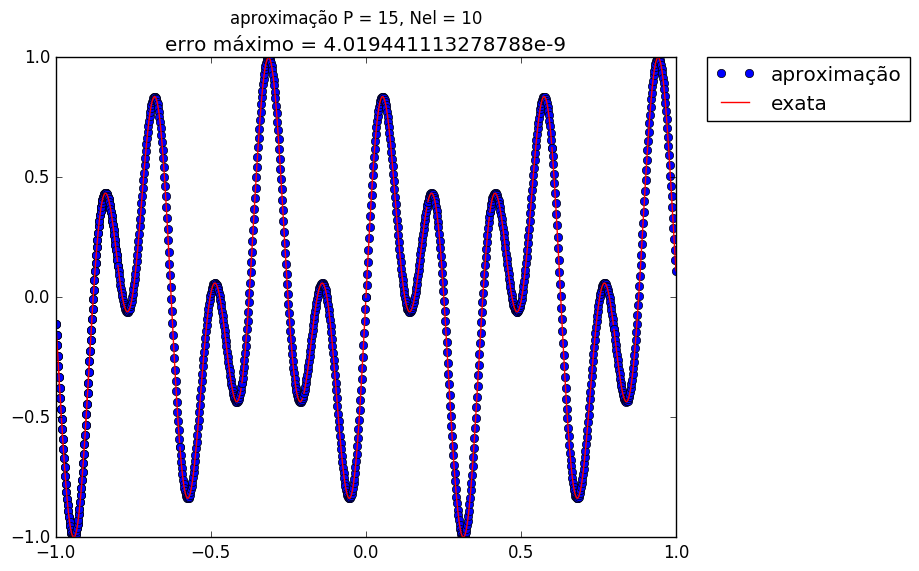
\includegraphics[width=0.7\textwidth,center]{figuras/Neumm_10_15.png}
\caption{comparação entre a solução exata e a aproximada usando P = 15 e $N_{el} = 10$ } 
\end{figure}
A convergência dos erros utilizando o método P e o método H continuam semelhantes à convergência do erro dos métodos aplicado a condição de \emph{Dirichlet}:
\begin{figure}[H]
\centering
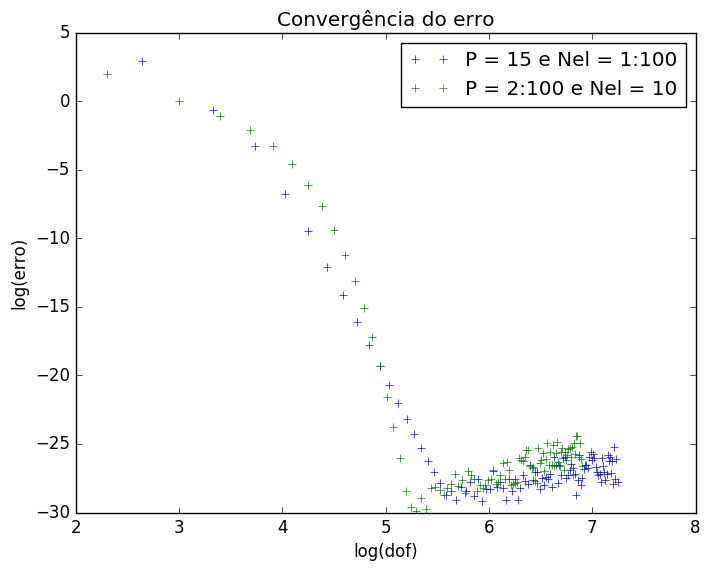
\includegraphics[width=0.7\textwidth,center]{figuras/convergencia_erro_Neumm.png}
\caption{convergência do log(erro) em função dos log(graus de liberdade) fixando o grau do polinômio em P e variando o número de elementos entre 1 a 40 } 
\end{figure}
 Agora veremos a convergência do erro para a aproximada da \emph{derivada} da solução no ponto onde temos a condição de \emph{Neumman} ocorre:
\begin{figure}[H]
\centering
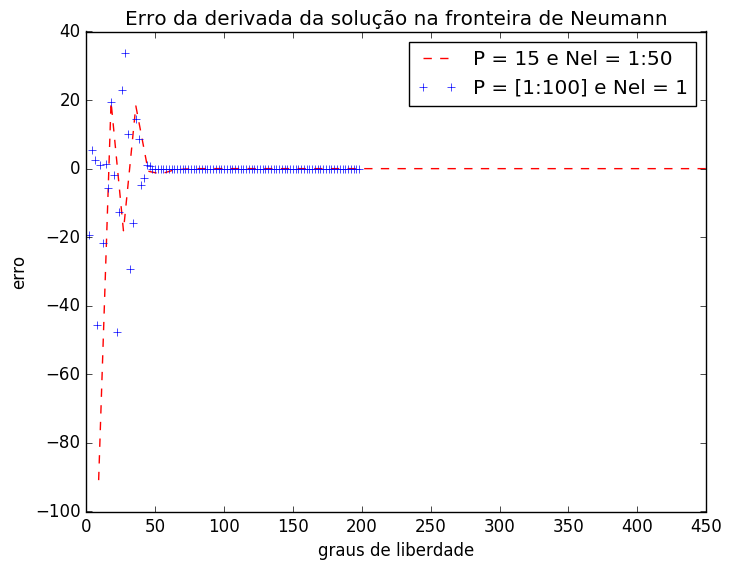
\includegraphics[width=.8\textwidth,center]{figuras/erro_derivada.png}
\caption{convergência do erro da derivada da solução aproximada entre os dois métodos} 
\end{figure}

\section{onde o método HP se sobrepõe?}
 Ao utilizar o método HP, estamos alternando entre os dois método. Notamos que para funções com alta frequência como a anterior caso utilizemos apenas o método P, teriamos que utilizar um polinômio de grau elevado para obter uma boa aproximação:
\begin{figure}[H]
\centering
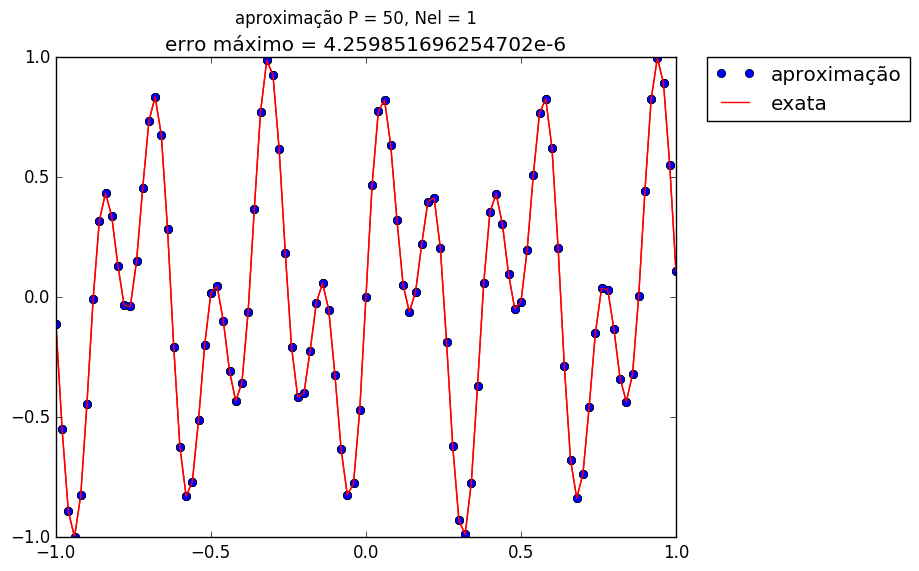
\includegraphics[width=0.8\textwidth,center]{figuras/Neumm_1_50.png}
\caption{aproximação do método P de grau 50} 
\end{figure}
 Agora, utilizando o método HP, utilizamos um polinômio de grau 20 e aumentando o número de elementos observamos o quanto o erro converge rapidamente:\begin{figure}[H]
\centering
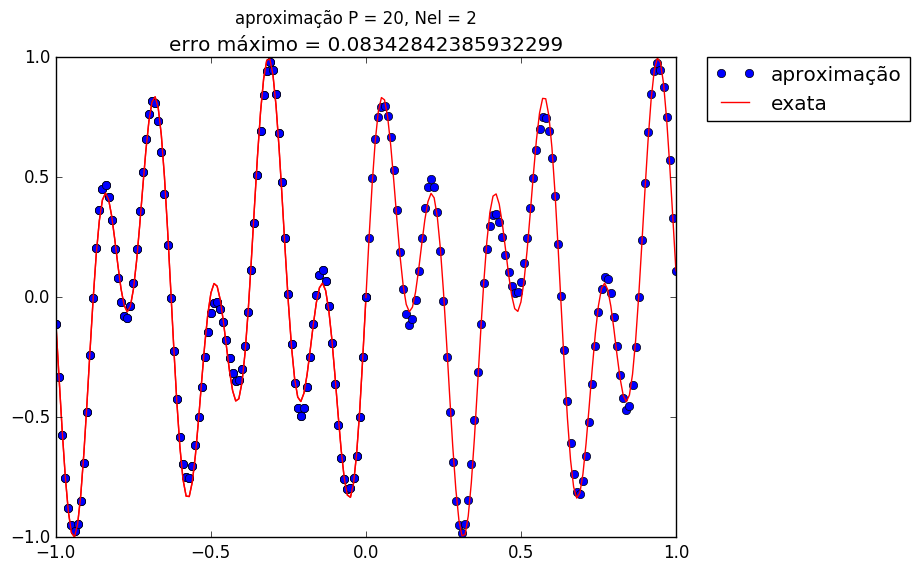
\includegraphics[width=0.7\textwidth,center]{figuras/Neumm_2_20.png}
\caption{aproximação do método P de grau 20 e $N_{el} = 2$} 
\end{figure}
\begin{figure}[H]
\centering
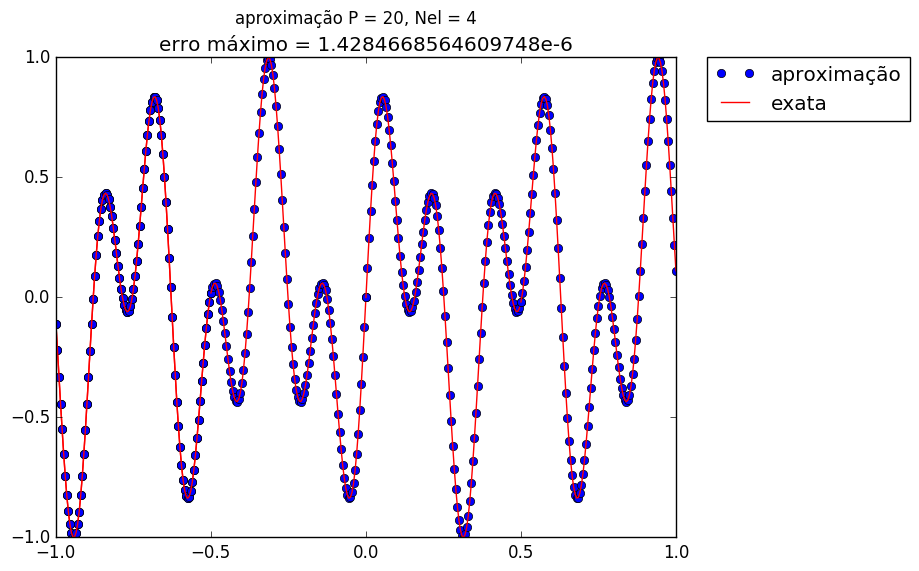
\includegraphics[width=0.75\textwidth,center]{figuras/Neumm_4_20.png}
\caption{aproximação do método P de grau 20 e $N_{el} = 4$} 
\end{figure}

Assim, para um melhor aproveitamento do método, temos que para funções mais complexas, o uso de apenas um polinômio de grau elevado não é muito proveitoso para a minimização  do erro. Portanto subdividindo o problema em elementos, facilita uma melhor a aproximação da solução do problema.